\documentclass[review]{elsarticle}
\usepackage{hyperref}
\usepackage[margin=1in]{geometry}
\usepackage{graphicx}
\usepackage{amsmath}
\usepackage{placeins}
\usepackage{comment}
\usepackage{gensymb}
\usepackage{lineno}
\usepackage{flexisym}
\usepackage{color}
\usepackage[title]{appendix}

\journal{Journal of Nuclear Materials}
\bibliographystyle{elsarticle-num}

\begin{document}

\begin{frontmatter}
\title{\textit{Ab initio} molecular dynamics investigation of point defects in $\gamma$-U}

\author[ncsu,inl]{Benjamin Beeler\corref{qwe}}
\cortext[qwe]{Corresponding author}
\ead{bwbeeler@ncsu.edu}
\author[lanl]{David Andersson}
\author[inl]{Chao Jiang}
\author[wisc,inl]{Yongfeng Zhang}
\address[ncsu]{North Carolina State University, Raleigh, NC 27607}
\address[inl]{Idaho National Laboratory, Idaho Falls, ID 83415}
\address[lanl]{Los Alamos National Laboratory, Los Alamos, NM 87545}
\address[wisc]{University of Wisconsin-Madison, Madison, WI 53706}

\begin{abstract}

Uranium (U) is often alloyed with molybdenum (Mo) or zirconium (Zr) in order to stabilize the high-temperature body-centered cubic $\gamma$ phase of uranium for use in nuclear reactors. However, relatively little experimental or computational investigation has centered on $\gamma$-U, largely due to the mechanical instability of this phase at room temperature. This is particularly problematic for density functional theory calculations that typically investigate 0 K properties. However, \textit{ab initio} molecular dynamics (AIMD) allows for quantum mechanical-based calculations to be performed at non-zero temperatures. In this work, AIMD simulations are performed to calculate the equilibrium volume for the $\gamma$ phase of U from 900 K to 1400 K. Utilizing the volume at each temperature, the bulk modulus, the radial distribution function, the interstitial and vacancy formation energies, and the diffusion coefficients are determined. This is the first AIMD investigation of point defects in $\gamma$-U. 

\end{abstract}
\end{frontmatter}

\section{Introduction}

Uranium (U) is an actinide exhibiting delocalized f-electrons that exists in three solid phases: $\alpha$ (face-centered orthorhombic), $\beta$ (body-centered tetragonal) and $\gamma$ (body-centered cubic) \cite{yoo1998}. At elevated temperatures, U transforms from $\alpha$ to $\beta$ at approximately 935 K and $\beta$ transforms to $\gamma$ at approximately 1045 K \cite{soderlind1998}. Uranium is alloyed with Mo or Zr in order to stabilize the preferred body-centered cubic phase to lower temperatures, most notably for application as nuclear fuel. 

Density functional theory (DFT) is an essential part of computational materials science, addressing a variety of problems in materials design and processing on a fundamental level. Several examinations of U via DFT have been performed on the orthorhombic and body-centered cubic (bcc) structures of U. Taylor \cite{taylor2008} used a projector augmented wave (PAW) pseudopotential to calculate the lattice constants of $\alpha$-U and $\gamma$-U along with the bulk modulus of both phases. Xiang, \textit{et al.} \cite{xiang2008} also utilized a PAW pseudopotential to perform an analysis of bulk properties in the $\alpha$ and $\gamma$ phases, as well as an analysis of defects in $\gamma$-U.  Beeler, \textit{et al.} calculated the lattice constants and elastic constants of $\alpha$, $\beta$ and $\gamma$-U \cite{beeler2013}, in addition to the point defect properties in both $\alpha$ and $\gamma$-U \cite{beeler2010}. Huang and Wirth \cite{wirth2011, wirth2012} calculated intrinsic and extrinsic point defect formation energies and migration barriers in $\alpha$-U. These DFT investigations showed a general, if imperfect, agreement with the experimental bulk moduli, lattice and elastic constants and vacancy formation energy \cite{yoo1998, barrett1963, matter1980}. 

The explanation for such a limited scope of analysis on the $\gamma$ phase lies partially in the inherent issues associated with a DFT approach to the study of a high temperature phase. DFT calculations are typically performed to calculate ground state properties, implying that the calculation is taking place at a temperature equal to 0 K. It has been shown, via the calculation of elastic constants, that the elastic shear constant (C\textprime=$\frac{1}{2}$(C$_{11}$-C$_{12}$)) is negative in the body-centered cubic phase of U \cite{soderlind1998, beeler2013}. Thus, at low temperatures $\gamma$-U is mechanically unstable. Computationally, this mechanical instability translates into an inability to calculate relaxed structures involving defects, due to the inherent localized deformation created by introducing a point defect that leads to deconstruction of the crystal lattice. Several other systems, such as Zr, Ti, and Hf, also exhibit a high temperature bcc phase that is mechanically unstable at low temperature \cite{sanchez1975, ye1987}. Beeler, \textit{et al.} \cite{beeler2010} attempted to circumvent this mechanical instability via the introduction of a ``shell" relaxation scheme, in which only a select group of atoms was permitted to relax around the defect. This methodology can provide an approximation for defect energies, but the accuracy of such a tactic is unclear. Additionally, this only provides an approximation for defect energies at 0 K and provides no insight into defect energetics at elevated temperatures and the extrapolation of properties at 0 K to high temperature systems is inexact at best.  

\textit{Ab initio} molecular dynamics (AIMD) allows for quantum mechanical-based calculations to be performed at non-zero temperatures. AIMD can account for the inherent anharmonicity responsible for making the bcc phase stable at high temperature, and as such allows for direct investigation of the bcc phase without any other required assumptions or restrictions.  AIMD has been utilized to study a variety of systems including liquid phase diffusion in Al-Si \cite{manga2018}, adsorption energy of Fe on TiN surfaces \cite{wang2010}, NaCl dissolution in water \cite{timko2010} and finite temperature phonon dispersion curves in bcc Zr and bcc Li \cite{hellman2011}. Hood, \textit{et al.} \cite{hood2008} have previously utilized AIMD to study the equation of state of U and the variation in density of states for the liquid phase of U at two unique temperatures. Hood, \textit{et al.} utilized a unique pseudopotential that was presented in that same manuscript \cite{hood2008}. Soderlind, \textit{et al.} \cite{soderlind2012} utilized self-consistent \textit{ab initio} lattice dynamics (SCAILD) to study the high temperature stabilization of the $\gamma$-U phase by calculating phonon modes at 1100 K. There have been no investigations in the free energy via the temperature dependent effect potential (TDEP) technique \cite{hellman2013} nor any AIMD investigations into the defect formation energies in $\gamma$-U at high temperatures. 

In this work, AIMD simulations are performed to calculate the energy as a function of volume for the $\gamma$ phase of U from 900 K to 1400 K. Utilizing the equilibrium volume at each temperature, the bulk modulus, the radial distribution function, the interstitial and vacancy formation energies, and the diffusion coefficients are determined. This is the first AIMD investigation of point defects in $\gamma$-U. 

\section{Computational Details}
Systems are investigated using the Vienna \textit{ab initio} Simulation Package (VASP) \cite{vasp1, vasp2, vasp3, vasp4}. The projector augmented wave (PAW) method \cite{paw1, paw2} is utilized within the density functional theory \cite{dft1, dft2} framework. Calculations are performed using the Perdew-Burke-Ernzerhof (PBE) \cite{pbe1, pbe2} generalized gradient approximation (GGA) density functional implementation for the description of the exchange-correlation. A uranium PAW pseudopotential with the 6s$^{2}$6p$^{6}$5f$^{3}$6d$^{1}$7s$^{2}$ valence electronic configuration and a core represented by [Xe, 5d, 4f] is utilized. Methfessel and Paxton's smearing method \cite{methfessel} of the first order is used with a width of 0.2 eV to determine the partial occupancies for each wavefunction. A Monkhorst-Pack \cite{monkhorst} 1x1x1 k-point mesh was utilized for Brillouin zone sampling. Uranium is assumed to be non-magnetic, in accordance with both experiments and previous simulations, and as such calculations are non spin polarized. The precision is set to normal and the energy cutoff is increased to 300 eV. The electronic self-consistent loop exit criterion is set to 10$^{-4}$ and the precision for projectors in real space is increased to -1E-4. A 128 atom supercell (4x4x4 unit cells) is utilized for all simulations. Dynamics were carried out in the NVT ensemble with a Nose-Hoover thermostat to control temperature, calculating both the forces and the stress tensor. The Nose mass was set to 0, allowing a period of 40 time steps. The timestep is set to 2.5 fs, and the simulation is carried out for 2000 timesteps (5 ps). In order to obtain average properties over the \textit{ab initio} molecular dynamics simulation, the energies and pressures for the final 1000 timesteps are extracted and averaged. The trajectories of the total supercell energy and pressure as a function of time step for an example simulation are shown in Fig. \ref{fig:convergence}. The energy and pressure both converge relatively quickly to a given value, with the energy oscillating by approximately $\pm$ 2 eV while the pressure oscillates by approximately $\pm$ 5 kB throughout the simulation. Given that there remains sufficient statistical scatter, an additional five unique simulations are performed with different random seeds in order to ensure statistical significance of the results. The system is verified to remain bcc by averaging the positions of the atoms over the final 1000 timesteps and performing a common neighbor analysis with the Ovito \cite{ovito} visualization software. 

\begin{figure}[h]
 \centering
 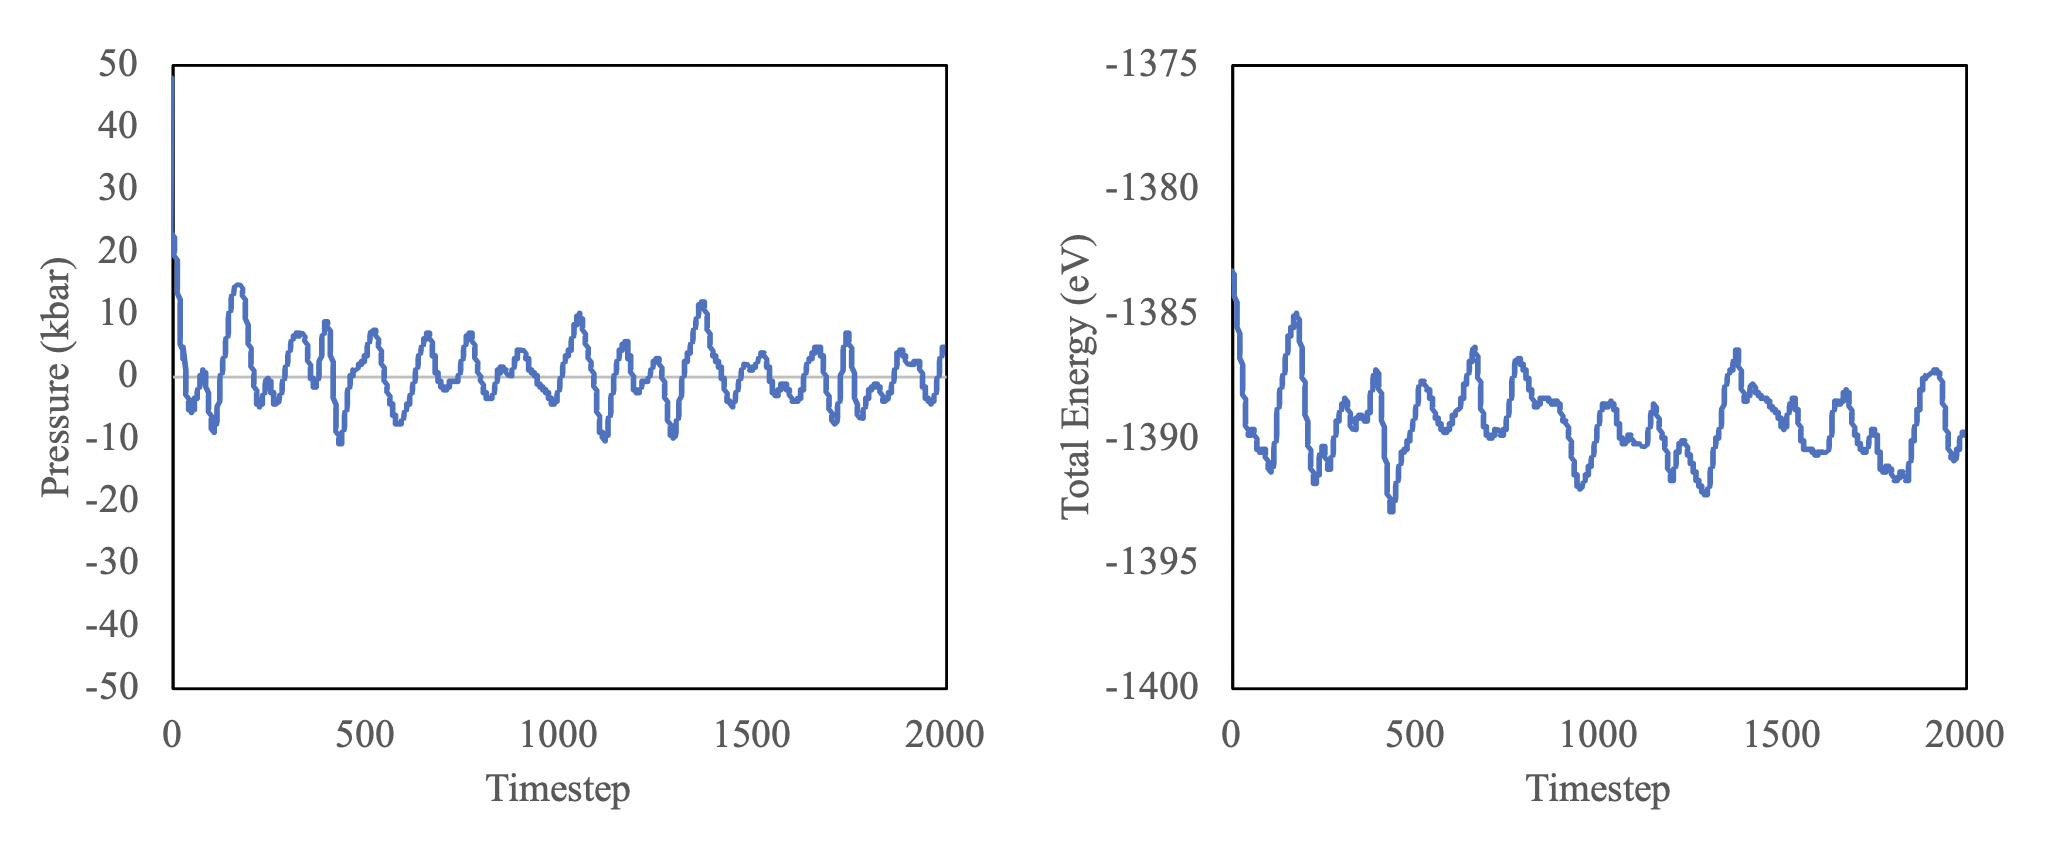
\includegraphics[width=0.95\textwidth]{1_convergence.png} 
 \caption{An example total supercell energy and pressure as a function of time. Data is extracted and averaged over the final 1000 timesteps to determine an energy and pressure for a given system. }
 \label{fig:convergence}
\end{figure}

\FloatBarrier

The system was evaluated at a series of volumes in order to construct a pressure as a function of volume (P(V)) relationship. The lattice constant is varied from 3.47 {\AA} up to 3.53 {\AA} in increments of 0.01 {\AA}. The point at which the P(V) relationship is equal to zero is determined to be the equilibrium volume. Subsquently, a second order polynomial function is fit to the dataset. Simulations were conducted for temperatures from 900 K up to 1400 K, in increments of 50 K. The melting point of uranium is 1408 K and the phase transition temperature into the $\gamma$ phase is 1045 K, thus this set of temperatures spans the entire range of stability for the $\gamma$ phase as well as exploring lower temperatures where the $\gamma$ phase is stable, but is not the equilibrium structure. The bulk modulus can be determined by taking the first derivative of pressure versus volume relationship with respect to volume:

\begin{equation}
\label{eq:bulk}
B_{0} = -V_0 \left( \frac{\partial P}{\partial V} \right)
\end{equation}

where B$_0$ is the bulk modulus, V$_0$ is the equilibrium volume, P is the pressure and P(V) is taken as the second order polynomial function to determine the bulk modulus. This calculated bulk modulus in input into the second order constant temperature Birch-Murnaghan equation of state (EOS) in equation \ref{eq:eos}.
\begin{equation}
\label{eq:eos}
P(V) = \frac{3B_0}{2} \left[ \left(\frac{V_0}{V}\right)^{\frac{7}{3}} - \left(\frac{V_0}{V}\right)^{\frac{5}{3}} \right]
\end{equation}

The formation energy of point defects is calculated via equation \ref{eq:eform}: 

\begin{equation}
\label{eq:eform}
E_f = E^* - \frac{n \pm 1}{n} \times E_0
\end{equation}

where E$^{*}$ is the energy of a system with a defect (with n $\pm 1$ atoms), \textit{n} is the number of atoms in the defect-free system and E$_{0}$ is the energy of a defect-free system with \textit{n} atoms. Equation \ref{eq:eform} utilizes (\textit{n} + 1) for interstitials and (\textit{n} - 1) for vacancies. All defect properties are determined in constant volume systems, set to the equilibrium volume for a given temperature. For systems involved in defect formation energy calculations, the number of simulations is increased from five to fifty, in order to improve the statistical significance of the results.

The diffusion coefficients for individual point defects and for self-diffusion in $\gamma$-U were determined by calculation of the mean-squared displacement (msd or $\langle$r$^2$$\rangle$) of atoms. A single point defect is inserted into the 128 atom supercell, the system is equilibrated for 2.5 ps. The system is then allowed to evolve for 22.5 ps, over which the msd is calculated. The diffusion coefficient is determined from the Einstein formula (D=$\langle$r$^2$$\rangle$/6t), where \textit{t} is the time. The slope of the msd versus time ($\langle$r$^2$$\rangle$/t) is taken as a linear fit to the complete dataset during the 22.5 ps relaxation, with data collected every 100 timesteps (0.25 ps). Five unique systems are investigated for each defect type and temperature in order to gain some statistical significance of the diffusion data. Select systems were investigated for convergence testing, in that a) the system simulation time is increased to 47.5 ps (from 22.5 ps), or b) the number of unique systems is increased from five to ten. No statistically significant difference was observed in either of these cases, and as such our methodology was deemed valid. 

The computational expense associated with these kinds of investigations should be emphasized. Nearly 2.5 million cpu-hours on a high-performance computing system were required to obtain the data within this manuscript, not including the intensive scoping and convergence testing that was performed. Ideally, additional simulations would be performed to increase the statistical accuracy of the results. However, the accuracy was deemed sufficient to provide meaningful results (as will be shown), taking into account the computational expense associated with increasing statistical significance. 

\section{Results}
\subsection{Equilibrium properties of $\gamma$-U}

The pressure as a function of volume for $\gamma$-U from 900 K to 1400 K is shown in Fig. \ref{fig:pvsv}, with the parametrized second-order Birch-Murnaghan equation of state (EOS) for each temperature. It should be noted that the pressure as a function of volume was calculated in increments of 50 K, but only 100 K increments are shown for clarity. The equilibrium lattice constant as a function of temperature is included in the appendix. The equilibrium volume is taken as the zero-crossing of each curve at a given temperature, and additional data points are included near the equilibrium volume. It can be observed that volumetric expansion takes place over this temperature range, as would be expected. Both Touloukian \cite{touloukian} and Basak \cite{basak} experimentally determined thermal expansion for $\gamma$-U and produced an empirical fit as a function of temperature, which can be translated into a linear thermal expansion (LTE) coefficient. The data from Touloukian leads to a LTE of 22.4 x 10$^{-6}$ K$^{-1}$ and the work of Basak lead to a LTE of 13.3 x 10$^{-6}$ K$^{-1}$, although the data from Basak is over a smaller temperature range. A comparison of the data calculated in this work to the experimental data is shown in Fig. \ref{fig:exp}. The thermal expansion is taken with respect to a system at 1100 K in order to compare with the experimental data, thus the expansion at 1100 K is zero. The AIMD simulations under-predict the thermal expansion compared to Touloukian, while exactly matching the values of Basak on the limited temperature range of 1100 - 1200 K. When including the entire temperature range from the AIMD calculations, the calculated of the LTE of 14.3 x 10$^{-6}$ K$^{-1}$, which again compares favorably with Basak and underestimates Touloukian.

The lattice constant is also underestimated when compared to experiment. At 1060 K, Lawson \cite{lawson1988} found the lattice constant to be 3.53 {\AA}, while this work predicts 3.493 {\AA} (at 1050 K). Previous DFT work has shown that the lattice constant of $\gamma$-U is underestimated compared to experimental values, however when those experimental values are extrapolated to 0 K, the results shown an overprediction of the lattice constant\cite{beeler2010, xie2013}. Utilizing a Hubbard U parameter within DFT has been shown to increase the lattice constant of $\gamma$-U \cite{xie2013}, and as such it is possible that AIMD with the inclusion of the Hubbard U parameter would yield equilibrium volumes that more closely match the experimental values, although this is not a sufficient argument to use the Hubbard U parameter. Also, it has been shown that for metallic U, a Hubbard U parameter is not required \cite{wirth2012, wirth2011, beeler2010, taylor2008, beeler2013} and is unclear what the effect of the Hubbard U parameter would be on other properties of interest. 

\begin{figure}[h]
 \centering
 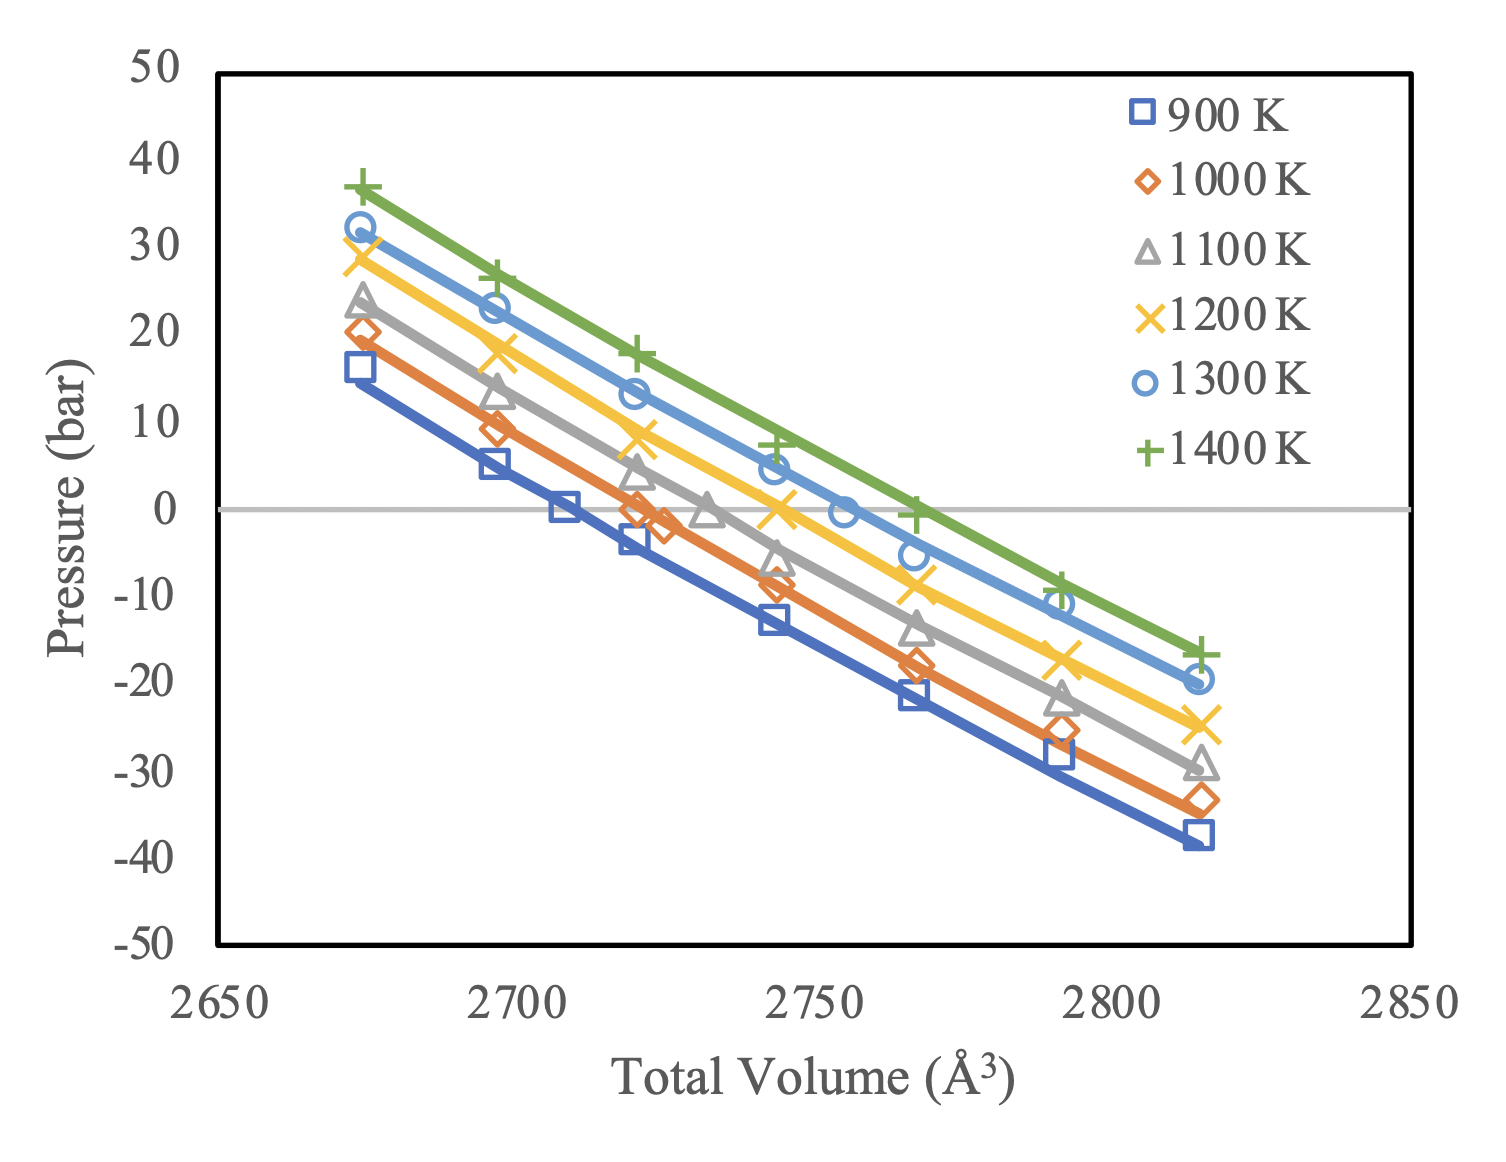
\includegraphics[width=0.75\textwidth]{2_p_vs_v.png} 
 \caption{The energy per atom as a function of volume for $\gamma$-U from 900 K to 1400 K. Lines are the parametrized second-order Birch-Murnaghan equation of state (EOS). Data included as open symbols. }
 \label{fig:pvsv}
\end{figure}

\begin{figure}[h]
 \centering
 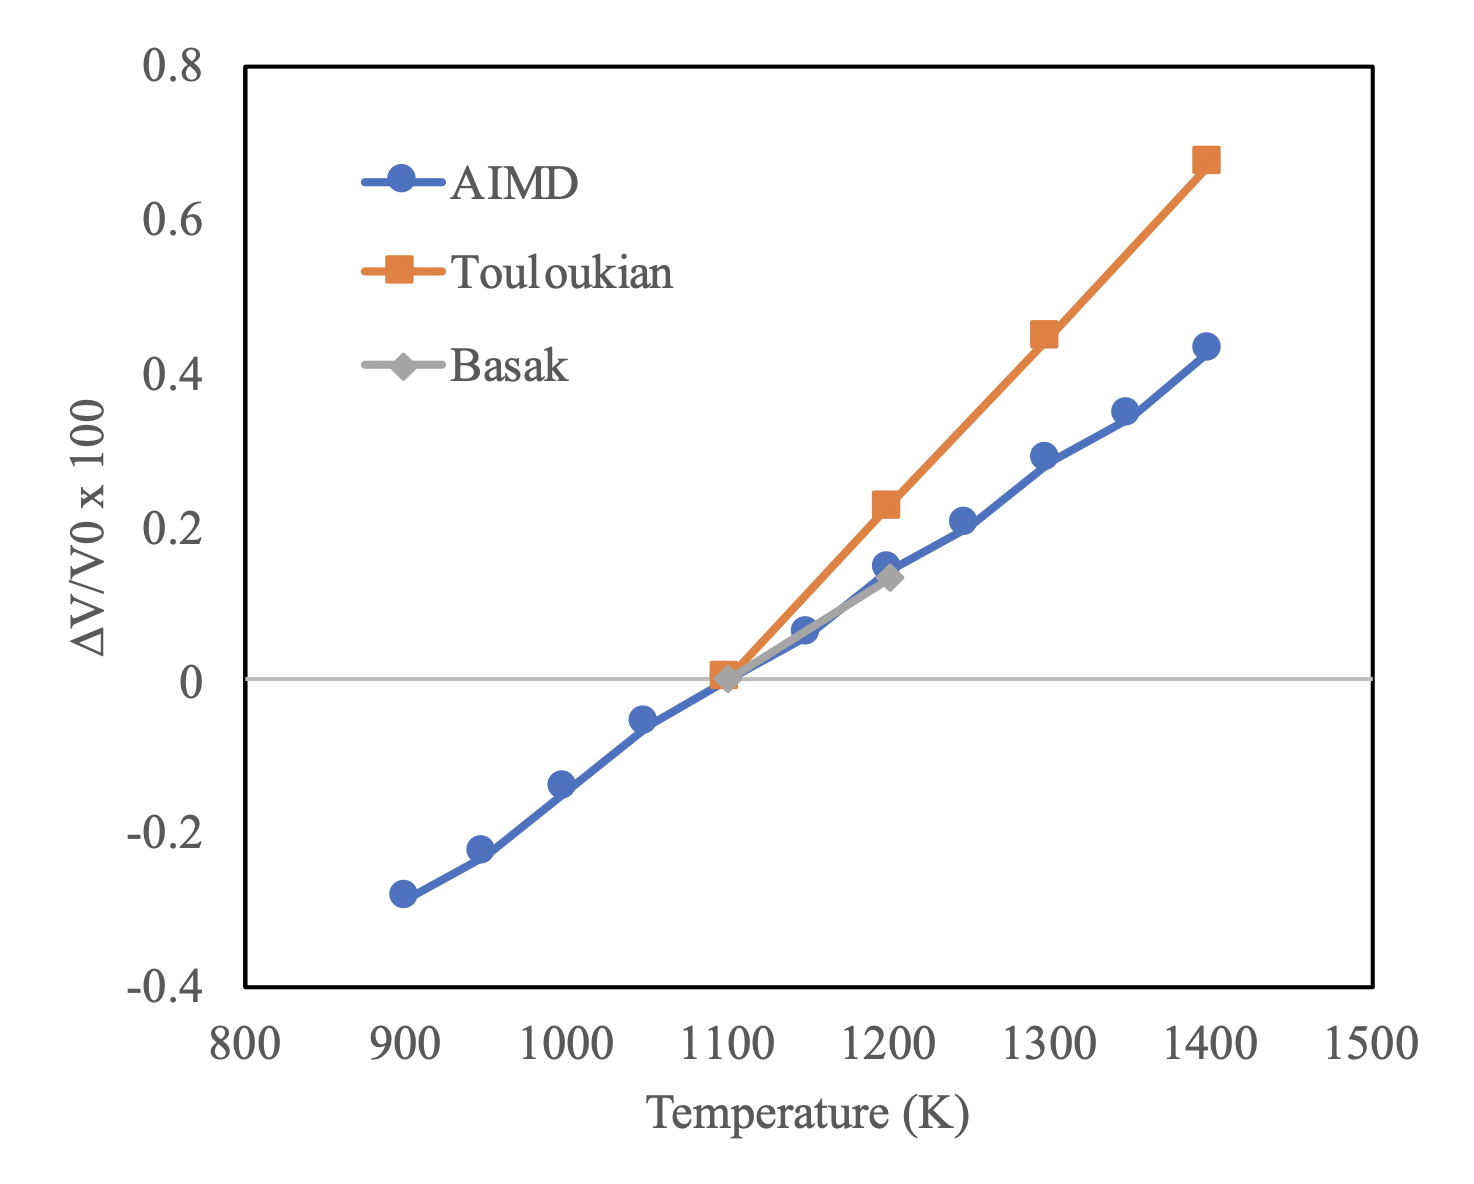
\includegraphics[width=0.75\textwidth]{3_thermal_exp.png} 
 \caption{The thermal expansion with respect to a system at 1100 K for this work (AIMD) and experimental work from Touloukian \cite{touloukian} and Basak \cite{basak} .   }
 \label{fig:exp}
\end{figure}

\FloatBarrier

The bulk modulus calculated from equation \ref{eq:bulk} is shown in Table \ref{tab:bulk}. Only increments of 100 K are shown for brevity, despite calculations at increments of 50 K. The full data is included in the appendix. There is a general softening of the bulk modulus with increasing temperature, as would be expected. An experimental value of the bulk modulus was calculated by Yoo \cite{yoo1998} as 113 GPa, utilizing a temperature independent equation of state. The values in this work are only slightly lower than the experimental work (by approximately 7 {\%}). This provides additional confidence in this methodology. Linearly fitting to the bulk modulus as a function of temperature shows that $\gamma$-U softens by approximately 2 GPa per 100 K. 

\begin{table}[h]
\caption{The bulk modulus of $\gamma$-U from 900 K to 1400 K.} \label{tab:bulk}
\begin{center}
\begin{tabular}{|c|c|}
	\hline
	Temperature (K) & Bulk Modulus (GPa) \\
	 \hline
	 900 & 108.1 \\
	 1000 & 109.4 \\
	 1100 & 105.1 \\
	 1200 & 103.6 \\	 
	 1300 & 98.5\\
	 1400 & 99.1 \\
	 \hline
\end{tabular}
\end{center}
\label{default}
\end{table}

\FloatBarrier

The radial distribution function (rdf or g(r)) is calculated at the equilibrium volume for each temperature and is displayed in Fig. \ref{fig:rdf}. The ideal bcc structure with a lattice parameter of 3.49 {\AA} is included for reference on a secondary axis. The rdf is determined from the average positions of the atoms in a given simulation, averaged over twenty unique snapshots. It is clear from Fig. \ref{fig:rdf} that the bcc structure is present for all temperatures, as the peak locations are exactly matched for all temperatures. However, at the low temperature regime near 900 K, additional peak roughening or broadening is observed, particularly for 1st, 3rd and 4th nearest neighbor peaks. This is exactly the opposite behavior of what would be expected, in that given the same crystal structure, the peaks should be narrower at lower temperatures and broader at higher temperatures due to increased thermal fluctuations. Thus, it is expected that 900 K is near the stability transition for the bcc structure of U and we are witnessing slight distortions away from the perfect bcc crystal structure. Above 1000 K, the rdf peaks more tightly fit the ideal bcc crystal structure.

\begin{figure}[h]
 \centering
 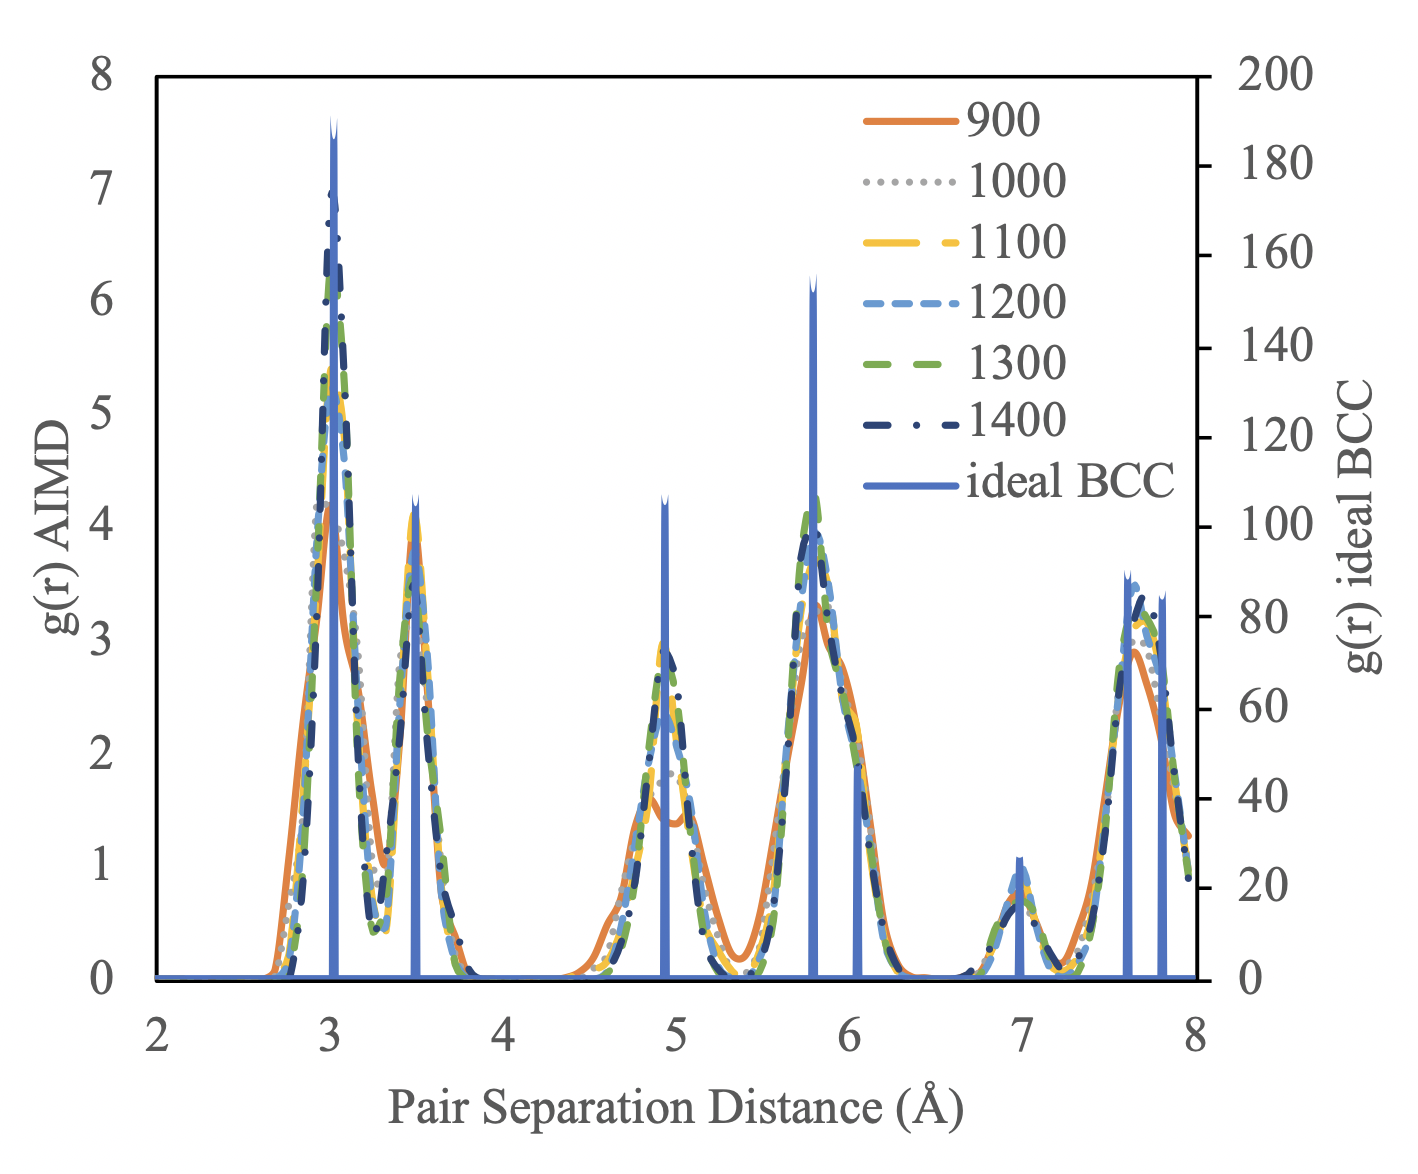
\includegraphics[width=0.8\textwidth]{4_rdf.png} 
 \caption{The radial distribution function (g(r)) for $\gamma$-U from 900 K to 1400 K. The ideal bcc structure with a lattice parameter of 3.49 {\AA} is included for reference on a secondary axis.  }
 \label{fig:rdf}
\end{figure}

\FloatBarrier

\subsection{Point Defect Energies of $\gamma$-U}

The point defect formation energy as a function of temperature is shown in Fig. \ref{fig:eform}. Data for both interstitials and vacancies is shown, with error bars representing plus/minus the standard error of the data set. The standard error for the formation energy is the sum of the standard error of the energy data set for a system with a point defect (E$^*$ in equation \ref{eq:eform}) and the standard error of the energy data set of a system with no defects (E$_0$ from equation \ref{eq:eform}). The full data is included in the appendix.

The first thing to note is that the interstitial formation energy is substantially lower than the vacancy formation energy across the entire temperature regime investigated. This is not the case in $\alpha$-U \cite{wirth2011} or in most metals \cite{schultz1968, baskes1979, lee2001, lee2003}, where the interstitial formation energy is substantially higher than the vacancy formation energy. However, this is in agreement with previous computational results \cite{beeler2010} as well as the experimental evidence suggesting that self-diffusion in $\gamma$-U is at least partially due to an interstitialcy mechanism \cite{fedorov1978, smirnov1992, mehrer2011}. The positron annihilation experimental investigations that have studied the vacancy formation energy in $\gamma$-U correspond with the magnitude of the vacancy formation energies from this work. Matter \cite{matter1980} reported a vacancy formation energy of 1.2$\pm$0.25 eV, while Lund \cite{lund2013} reported a value of 1.6$\pm$0.2 eV, although Lund suggested that oxygen impurities likely affected their results. There are no experimental results of interstitial formation energy for comparison.

The formation energy of both vacancies and interstitials increases with increasing temperature. This variance in vacancy formation energy has been previously shown computationally in Al by Carling \cite{carling2003} and in Fe and Zr by Mendelev \cite{mendelev2009, mendelev2010}, and for interstitials in Zr by Mendelev \cite{mendelev2010}. Defect behavior in U has been compared to Zr due to the hexagonal-type ground state structures for both elements paired with high temperature bcc structures which are mechanically unstable at lower temperatures, in addition to similar anomalous diffusive behavior \cite{matter1980,kidson1961}. The magnitude of increase (0.5 - 1 eV) observed in this work is in line with these previous studies. The ratio of the vacancy formation energy to the interstitial formation energy decreases slightly with increasing temperature.

The magnitude of the formation energies, particularly for interstitials, should be emphasized. This work compares very favorably to the previous DFT study on point defects in $\gamma$-U at 0 K\cite{beeler2010}, which showed the interstitial formation energy as low as 0.5 eV. Despite this agreement, the formation energies seem abnormally low.  Neglecting entropic effects, the formation energies at the provided temperatures would yield equilibrium interstitial concentrations on the order of 10$^{-3}$ defects per atom. Additionally, the inclusion of entropic effects should \textit{increase} the equilibrium defect concentrations. Typically such high defect concentrations are not observed except for very close to the melting point. However, this work suggests such defect concentrations are present across the entire temperature range of phase stability for the $\gamma$ phase (0.64T$_m$ - 1.0T$_m$). It has been shown that increasing defect concentration leads to a decrease in melting point \cite{sorkin2003}, and it is possible that the low interstitial formation energy in $\gamma$-U leads to the comparatively low melting of U compared to Zr or other bcc metals \cite{williams1990} such as Fe, V or Mo, which all have higher interstitial formation energies \cite{mendelev2010, mendelev2009, nguyen2006} as well as higher melting points. It is also possible that entropic effects play an important role in determining the equilibrium defect concentrations, or that the "perfect crystal" of $\gamma$-U contains point defects, or that investigating point defects in the dilute approximation with a pristine crystal has limited applicability in $\gamma$-U. It is regretfully beyond the scope of this work, and debatably beyond the scope of current computational capabilities, to thoroughly examine defect clusters in $\gamma$-U in an AIMD framework and obtain statistical significance. 

 \begin{figure}[h]
 \centering
 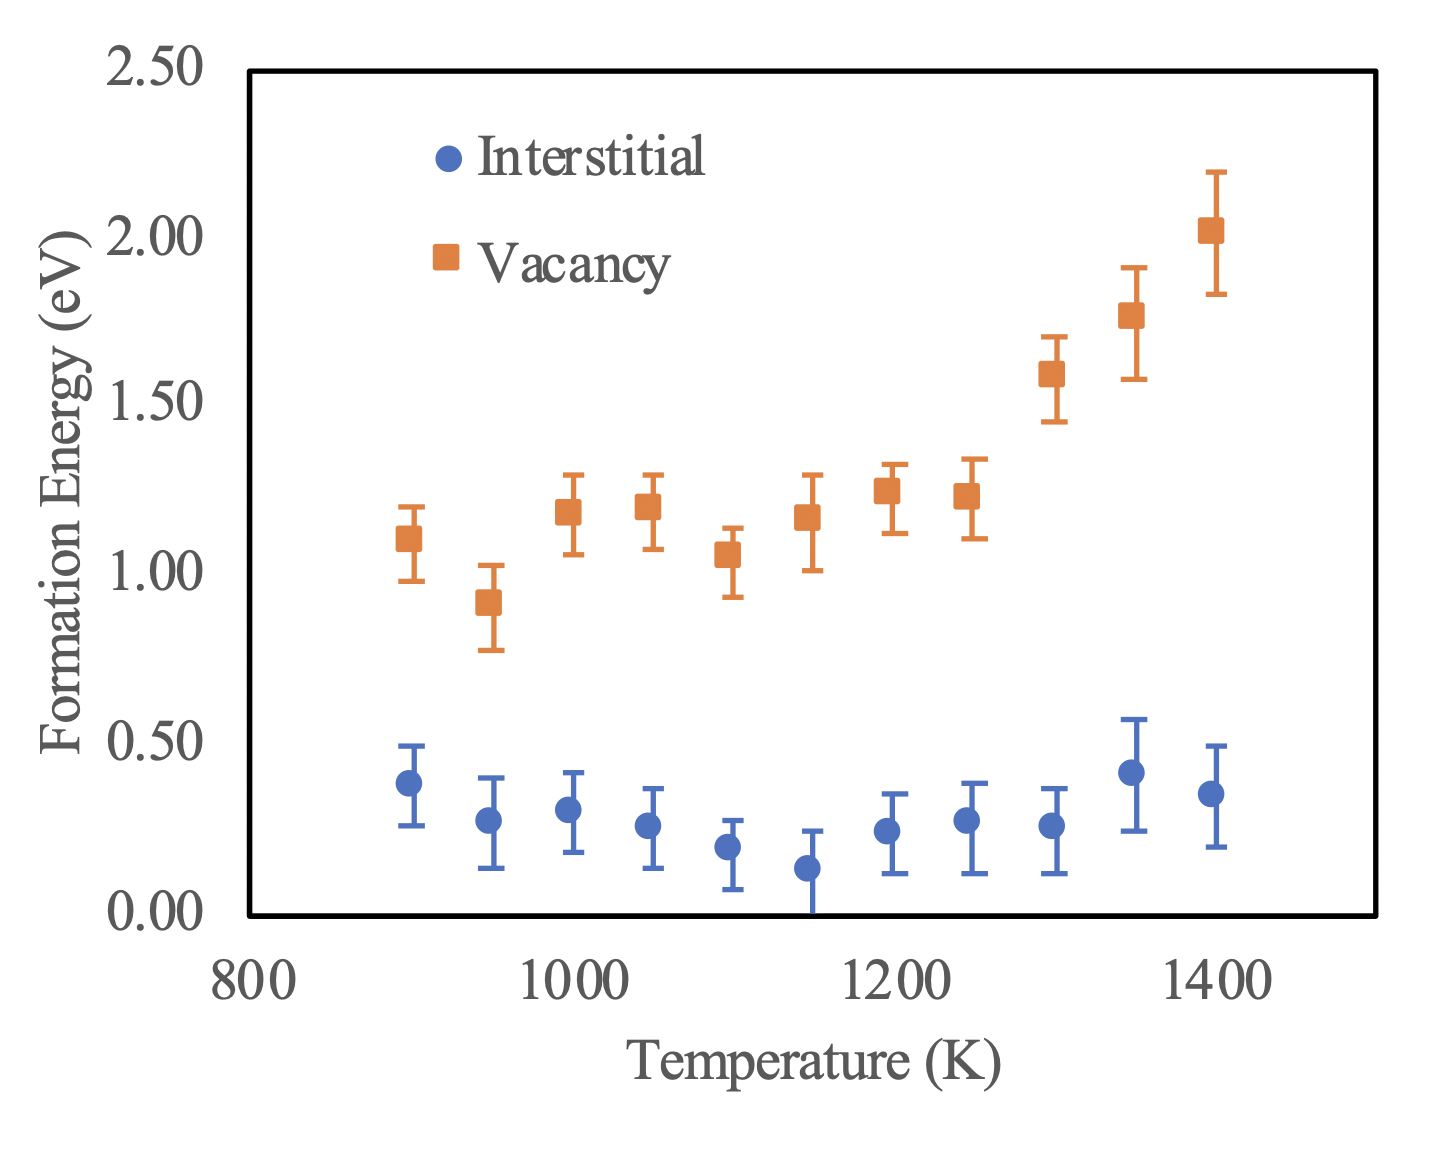
\includegraphics[width=0.75\textwidth]{5_eform.png} 
 \caption{The point defect formation energy for $\gamma$-U from 900 K to 1400 K. Error bars represent plus/minus one standard error of the data set. }
 \label{fig:eform}
\end{figure}



\FloatBarrier

\subsection{Point Defect Diffusion in $\gamma$-U}

The mean squared displacement ($\langle$r$^2$$\rangle$) as a function of time was tracked over 22.5 ps for systems with an individual point defect. The $\langle$r$^2$$\rangle$ data for interstitials and vacancies is shown in Fig. \ref{fig:rsquare}. Given that only five individual systems are utilized and that only a relatively short period of time is investigated, there is inherently some statistical fluctuation in the data. In spite of this, the $\langle$r$^2$$\rangle$ behavior is generally linear with time and diffusion coefficients can be estimated. To demonstrate that a number of jumps have taken place within a given system, trajectories generated from Ovito \cite{ovito} are shown for an interstitial and a vacancy at 1200 K in Fig. \ref{fig:traject}. It can be seen in both systems that a number of hops ($>$10) have taken place over the 22.5 ps of the simulation, with vacancy diffusion occurring along first nearest-neighbor pathways, and interstitial diffusion being more complicated, but similarly primarily along the $<$111$>$ directions. The majority of the atoms in the supercell remain oscillating about their original lattice position. Two things should be noted: 1) trajectories shown are smoothed over ten frames to generate a cleaner image, and the actual thermal fluctuations about the equilibrium lattice positions are substantially larger than shown, and 2) that periodic boundary crossings are occurring and the msd takes this into account. 



 \begin{figure}[h]
 \centering
 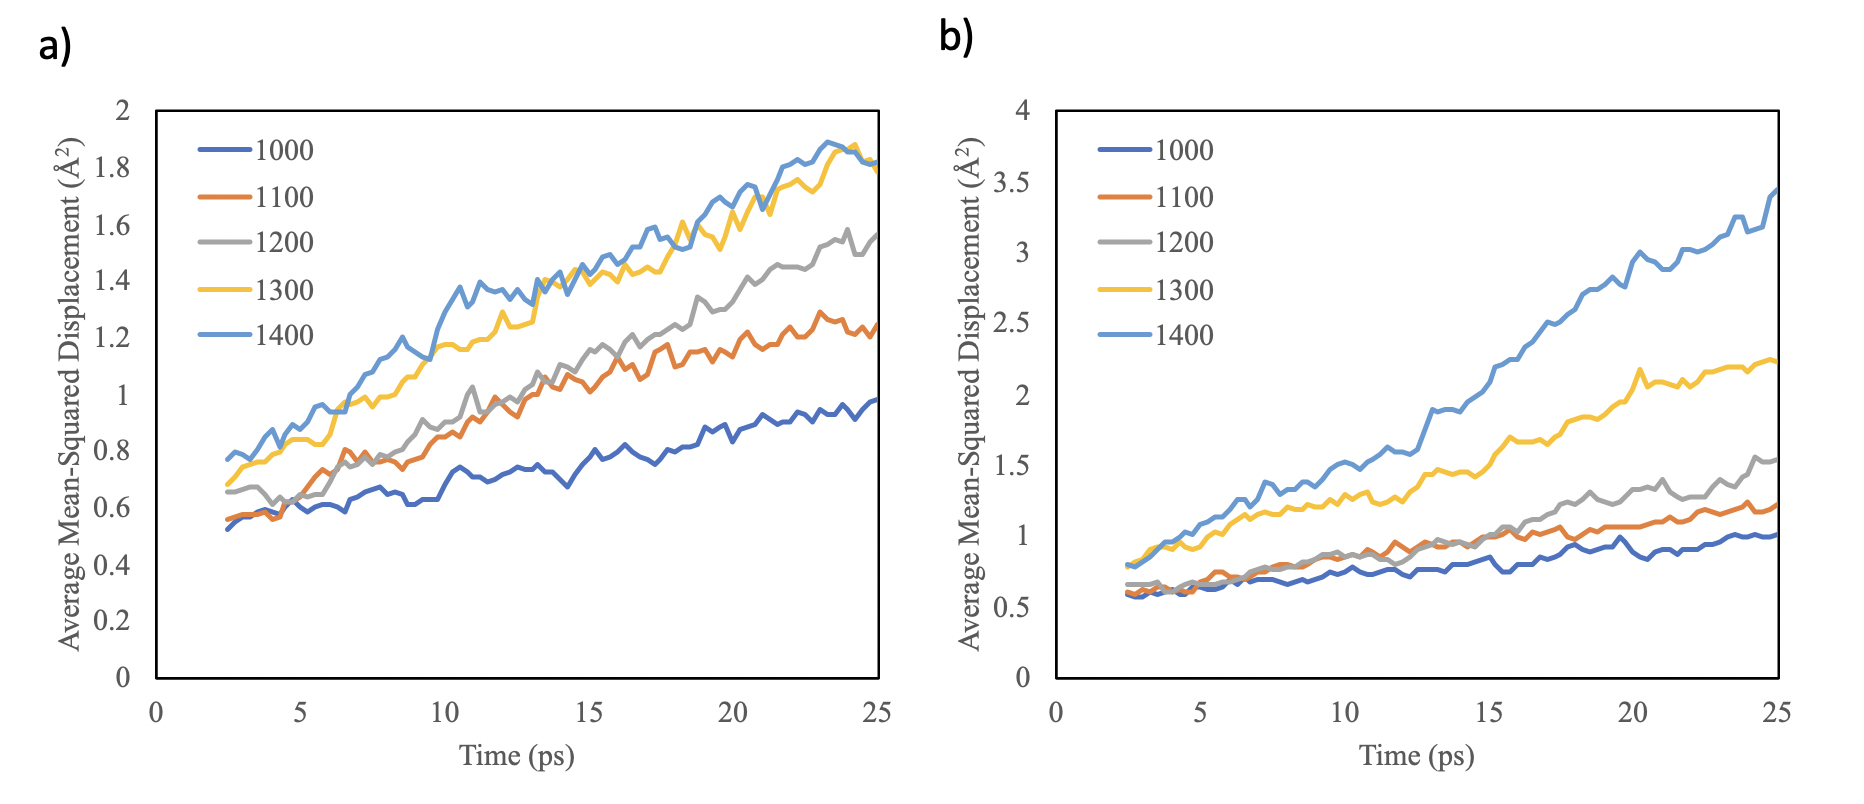
\includegraphics[width=0.9\textwidth]{6_msd.png} 
 \caption{The mean-squared displacement as a function of time for a) interstitials and b) vacancies from 1000 K to 1400 K.  }
 \label{fig:rsquare}
\end{figure}

 \begin{figure}[h]
 \centering
 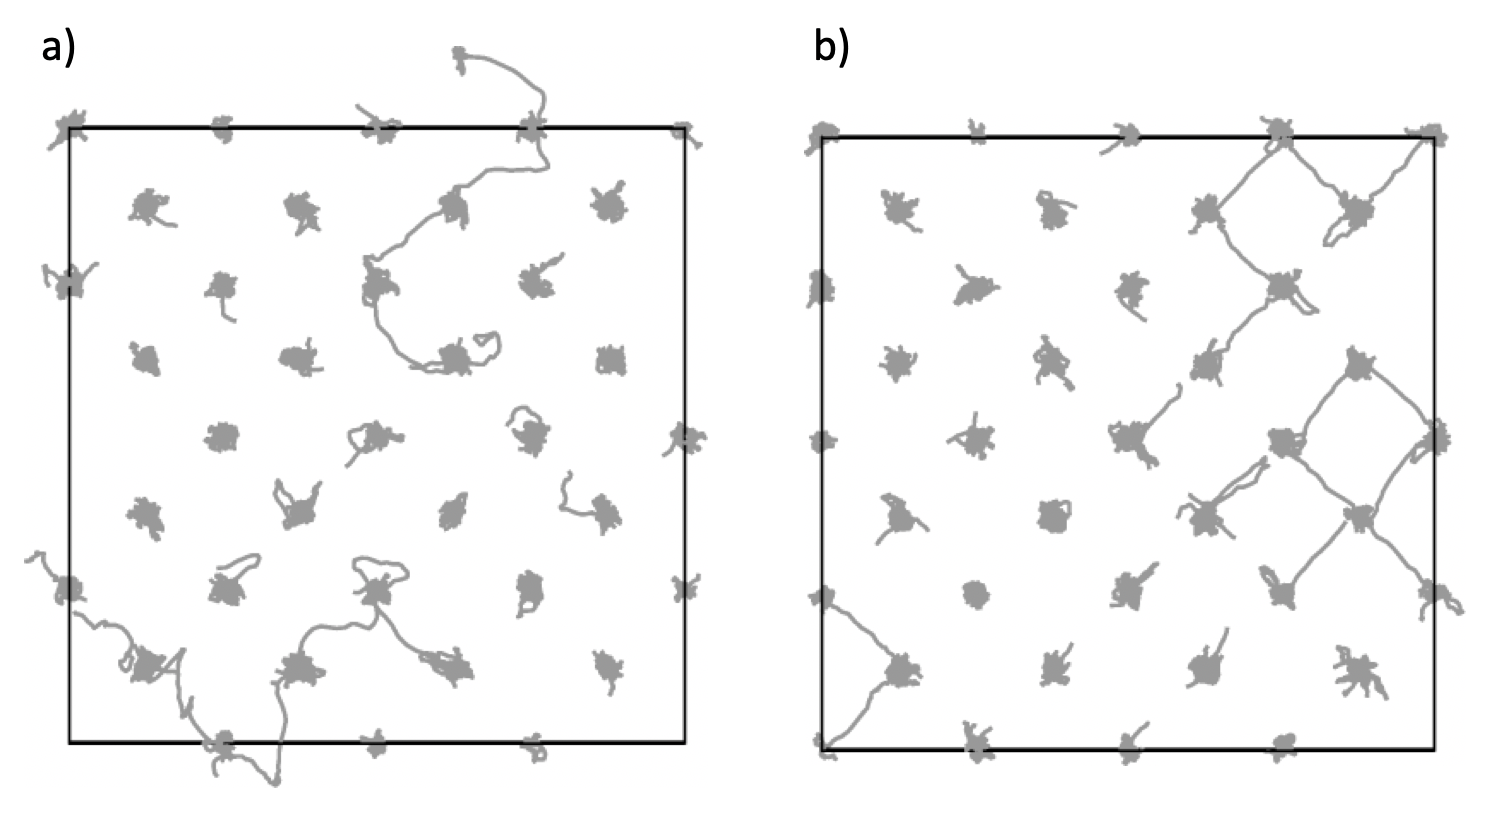
\includegraphics[width=0.9\textwidth]{7_trajectories.png} 
 \caption{The trajectories over time for a) interstitials and b) vacancies at 1200 K. Atoms have been removed so as to better illustrate the trajectories. Images are of the (100) plane. }
 \label{fig:traject}
\end{figure}

\FloatBarrier

The calculated diffusion coefficients for vacancies and interstitials are shown in Fig. \ref{fig:diff}, with exponential fits to the individual data sets are included as dashed lines. It can be seen that the diffusion coefficient for interstitials and vacancies exhibits a similar magnitude, albeit unique slopes. This study shows that the vacancy displays a slightly higher migration barrier than the interstitial, which leads to the vacancy diffusion coefficient being higher than the interstitial diffusion coefficient in the high temperature regime (1200-1400K) but lower than the interstitial diffusion coefficient in the low temperature regime (900-1100K).  An exponential function can be fit to the data to obtain a pre-factor and a migration barrier for each point defect. This data is reported in Table \ref{tab:diff}. 

 \begin{figure}[h]
 \centering
 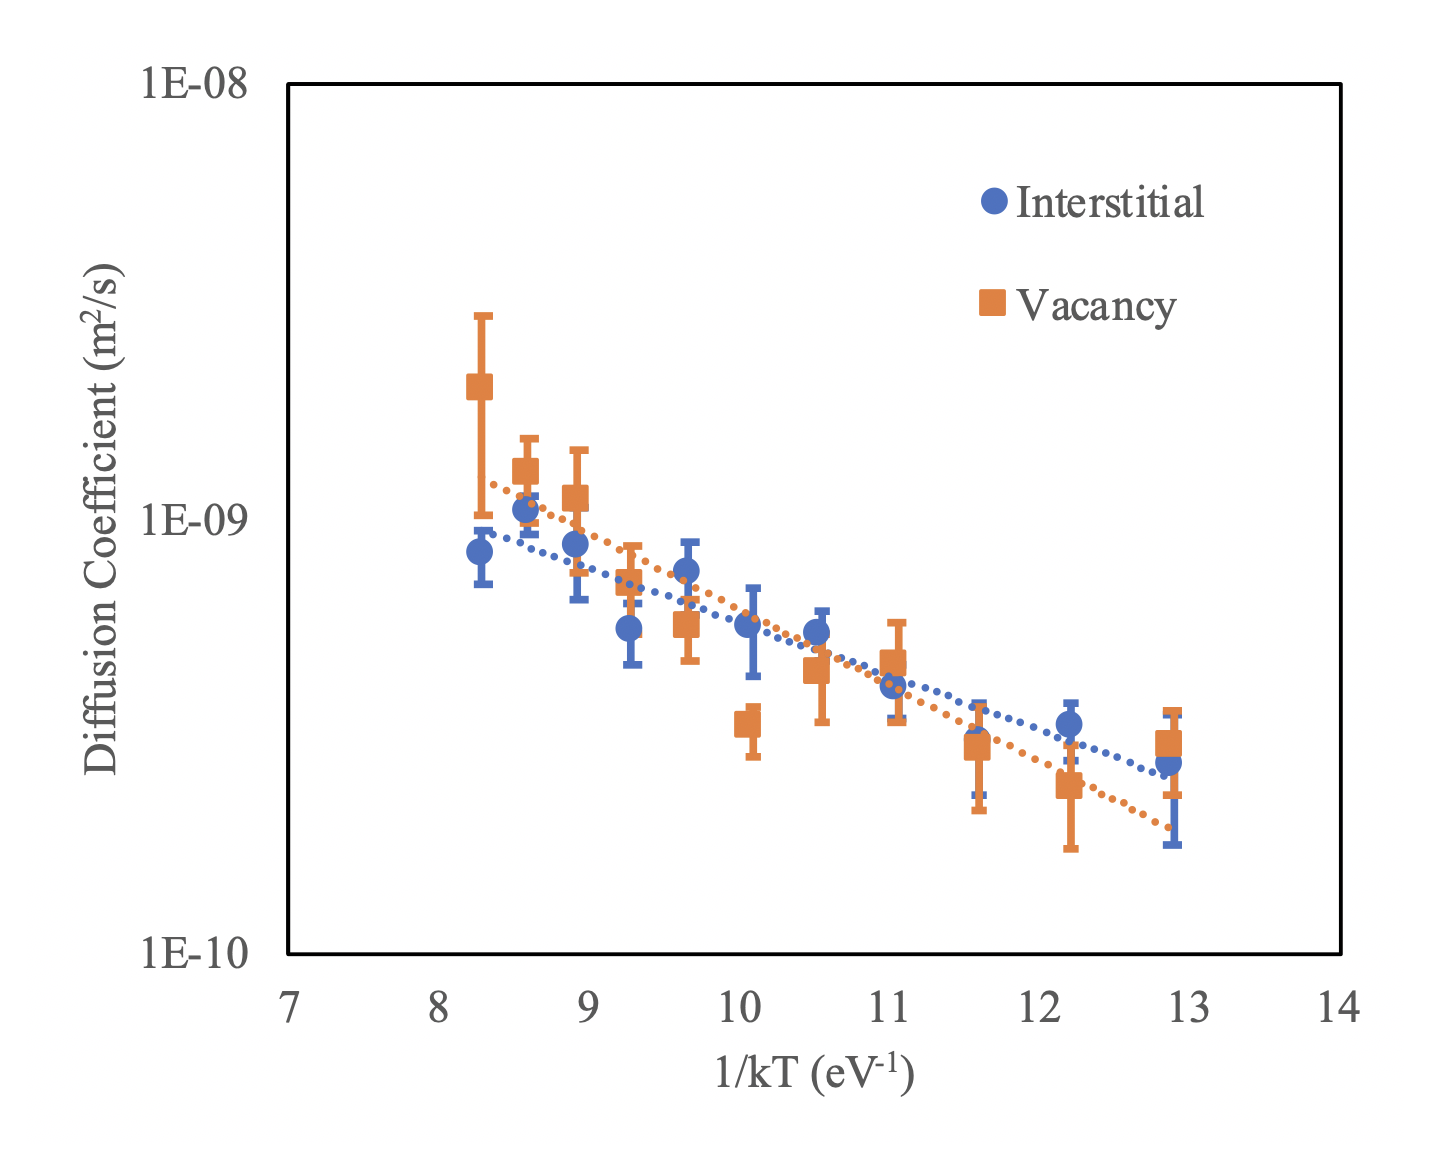
\includegraphics[width=0.75\textwidth]{8_diff.png} 
 \caption{The vacancy and interstitial diffusion coefficient for $\gamma$-U from 900 K to 1400 K. Exponential fits to the individual data sets are included as dashed lines.}
 \label{fig:diff}
\end{figure}

\FloatBarrier

\begin{table}[h]
\caption{The migration barrier (E$_m$) for vacancies and interstitials, the activation energy (Q$_A$) for self-diffusion and associated pre-factors in $\gamma$-U over the temperature range of 900 K - 1400 K.}  \label{tab:diff}
\begin{center}
\begin{tabular}{|c|c|c|}
	\hline
	 & E$_m$ or Q$_A$ (eV) & D$_0$ (m$^2$/s) \\
	 \hline
	 D$_{vac}$ & 0.40 & 3.52x10$^{-8}$ \\
	 D$_{int}$ & 0.29 & 9.99x10$^{-9}$ \\
	 D$_{self}$ & 0.59 & 1.00x10$^{-8}$ \\
	 \hline
\end{tabular}
\end{center}
\label{default}
\end{table}

In order to calculate a self-diffusion coefficient, an average defect formation energy is utilized (averaged from the data in Fig. \ref{fig:eform} from 900 K - 1400 K) for both a vacancy (1.3 eV) and an interstitial (0.3 eV). This is a simplification intended to acknowledge the lack of point defect entropies. Ideally, both temperature dependent point defect formation energies and entropies should be utilized. These formation energies are utilized in equation \ref{eqn:selfd}:

\begin{equation}
\label{eqn:selfd}
D_{self} = D_{int}c_{int} + D_{vac}c_{vac}
\end{equation} 

where D$_{int}$ and D$_{vac}$ are the diffusion coefficients from Table \ref{tab:diff} and c$_{int}$ and c$_{vac}$ are the interstitial and vacancy concentrations taken from \textit{exp}$(-E_{def}/kT)$, where $E_{def}$ is either the interstitial or vacancy formation energy averaged from Fig. \ref{fig:eform}. The entropic contribution on the defect concentration is assumed to be small and thus treated as a factor of one, given that there is no data on the entropic effects of point defects in $\gamma$-U. The calculated self-diffusion coefficient is displayed in Fig. \ref{fig:selfdiff}. Two experimental results are provided as a comparison \cite{rothman1959,adda1959}. Very little other experimental data is available for comparison and none after 1960, as such, further experimental studies are warranted. It can be seen that this work over-predicts the self-diffusion in $\gamma$-U compared to the existing experimental results by approximately one order of magnitude at 1400 K, and as much as two orders of magnitude at 1000 K. The self-diffusion coefficient is effectively solely due to interstitial diffusion, in that interstitial self-diffusion is approximately three to four orders of magnitude faster than vacancy self-diffusion. This is due to the much lower interstitial formation energy, despite the similar diffusion coefficients observed from Fig. \ref{fig:diff}. The activation energy (Q$_A$) from the experimental results are 1.19 eV \cite{adda1959} and 1.15 eV \cite{rothman1959}, while this AIMD work predicts an Q$_A$ of 0.59 eV. This is a substantial difference in the activation energy. The pre-exponential factor from this work is approximately an order of magnitude smaller than the experimental values (1.80E-7 \cite{adda1959} and 1.12E-7 \cite{rothman1959}, units in m$^2$/s). 

These discrepancies with the experimental literature can likely be explained by to the nature of dealing with pristine systems in a computational framework. Rothman \cite{rothman1959} reported that they created an ultra-high purity with a residual impurity composition in the range of 100-250 ppm by weight. Additionally, some mechanical processing, including rolling an annealing, was performed on the samples, leading to grain boundaries and a population of residual defects. The presence of sinks, as grain boundaries or dislocations or solute atoms, can dramatically reduce the self-diffusion coefficient, particularly in such a rapidly diffusing system as $\gamma$-U. The role of impurities, alloying elements, or interfaces in the system were beyond the scope of this study. However, given the expected inaccuracies in the AIMD simulations due to short times and limited sample size, the omission of actual defect entropies, and the inherent differences in experimental samples and ideal simulation environments, this is considered reasonable agreement and provides confidence in both the modeling methodology and the experimental results. The activation energy and pre-factor for self-diffusion are included in Table \ref{tab:diff}. 

It is recommended that these diffusion coefficients be utilized in conjunction with higher length scale modeling methodologies that are able to take into account defect interaction with sinks, or as representative of single crystal self-diffusion in ultra-high purity $\gamma$-U.

 \begin{figure}[h]
 \centering
 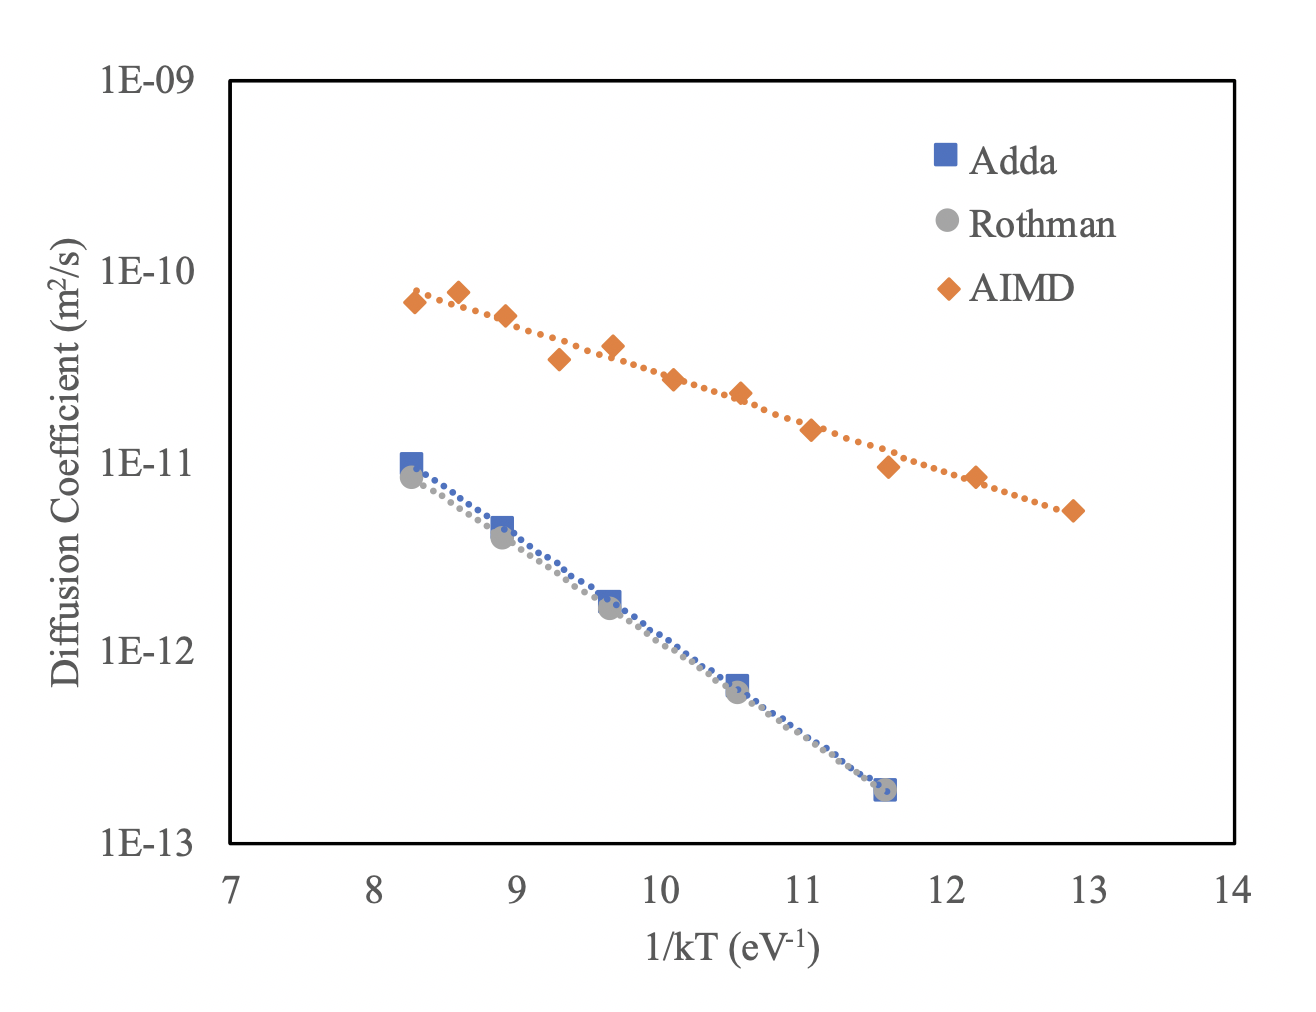
\includegraphics[width=0.75\textwidth]{9_self_diff.png} 
 \caption{The self-diffusion coefficient for $\gamma$-U from 900 K to 1400 K. Results are compared to experiments from Rothman \cite{rothman1959} and Adda \cite{adda1959}. }
 \label{fig:selfdiff}
\end{figure}

\FloatBarrier

\section{Conclusions}

In this study, AIMD simulations were performed to calculate the pressure as a function of volume for the $\gamma$ phase of U from 900 K to 1400 K. Utilizing the equilibrium volume at each temperature, the bulk modulus, the radial distribution function, the interstitial and vacancy formation energies, and the diffusion coefficients were determined. The lattice constant is slightly underestimated compared to experiment, while the thermal expansion and bulk modulus compare very favorably to data in the literature. The linear thermal expansion coefficient was found to be 14.3 x 10$^{-6}$ K$^{-1}$. The bulk modulus was observed to soften approximately 2 GPa per 100 K with increasing temperature. The calculated vacancy formation energies agree with the previous experimental results and both vacancy and interstitial formation energies agree with the previous computational studies. Point defect formation energies increase with increasing temperature, as has been reported in Zr and Al. The vacancy and interstitial diffusion coefficients, as well as the self-diffusion coefficient were calculated. The self-diffusion coefficient is overestimated and the activation energy is underestimated compared to experimentally reported results, presumably due to the lack of impurities or interfaces in the computational system. The magnitudes of the point defect formation energies in addition to the self-diffusion coefficients are consistent with the notion of self-diffusion via an interstitialcy mechanism in $\gamma$-U. 

This work has served to confirm the findings of previous studies regarding point defects in $\gamma$-U and provides further justification for describing self-diffusion in $\gamma$-U via an interstitialcy mechanism. This was the first \textit{ab initio} molecular dynamics study of point defects in $\gamma$-U and provides the foundation for expansion of computational studies at non-zero temperature in metallic U, with the inclusion of complex defects, interfaces, and impurities.

\section{Acknowledgement}
This work is supported by the U.S. Department of Energy, Office of Nuclear Energy, Nuclear Energy Advanced Modeling and Simulation (NEAMS) Program. This manuscript has been authored by Battelle Energy Alliance, LLC under Contract No. DEAC07-05ID14517 with the U.S. Department of Energy. The United States Government retains and the publisher, by accepting the article for publication, acknowledges that the United States Government retains a nonexclusive, paid-up, irrevocable, world-wide license to publish or reproduce the published form of this manuscript, or allow others to do so, for United States Government purposes.  Los Alamos National Laboratory, an affirmative action/equal opportunity employer, is operated by Los Alamos National Security, LLC, for the National Nuclear Security Administration of the U.S. Department of Energy under Contract No. DE-AC52-06NA25396.  This research made use of the resources of the High Performance Computing Center at Idaho National Laboratory, which is supported by the Office of Nuclear Energy of the U.S. Department of Energy and the Nuclear Science User Facilities under Contract No. DE-AC07-05ID14517.


\section{Data Availability}

The raw/processed data required to reproduce these findings cannot be shared at this time as the data also forms part of an ongoing study.

\begin{appendices}

\section{}

\setcounter{table}{0}
\renewcommand{\thetable}{A\arabic{table}}

\begin{table}[h]
\caption{The equilibrium lattice constant in $\gamma$-U from 900 K to 1400 K.} \label{tab:alat}
\begin{center}
\begin{tabular}{|c|c|c|}
	\hline
	Temperature (K) & a$_{0}$ ({\AA}) \\
	 \hline
900	&	3.485 \\
950	&	3.487 \\
1000	 &	3.490 \\
1050	 &	3.493 \\
1100	 &	3.495 \\
1150	 &	3.497 \\
1200	 &	3.500 \\
1250	 &	3.502 \\
1300	 &	3.505 \\
1350	 &	3.507 \\
1400	 &	3.510 \\
	 \hline
\end{tabular}
\end{center}
\label{default}
\end{table}

\begin{table}[h]
\caption{The bulk modulus in $\gamma$-U from 900 K to 1400 K.} \label{tab:bulkfull}
\begin{center}
\begin{tabular}{|c|c|c|}
	\hline
	Temperature (K) & B$_{0}$ (GPa) \\
	 \hline
900	&	108.1 \\
950	&	108.8 \\
1000	 &	109.4 \\
1050	 &	106.6 \\
1100	 &	105.1 \\
1150	 &	101.6 \\
1200	 &	103.6 \\
1250	 &	103.4 \\
1300	 &	98.5 \\
1350	 &	101.5 \\
1400	 &	99.1 \\
	 \hline
\end{tabular}
\end{center}
\label{default}
\end{table}


\begin{table}[h]
\caption{The point defect formation energy for vacancies (E$_{f}^{v}$) and interstitials (E$_{f}^{i}$) in $\gamma$-U from 900 K to 1400 K.} \label{tab:defs}
\begin{center}
\begin{tabular}{|c|c|c|}
	\hline
	Temperature (K) & E$_{f}^{v}$ (eV) & E$_{f}^{i}$ (eV) \\
	 \hline
  	   900 & 1.10 & 0.38 \\
	   950 & 0.91 & 0.27 \\
	 1000 & 1.18 & 0.31 \\
	 1050 & 1.19 & 0.26 \\
	 1100 & 1.05 & 0.18 \\
	 1150 & 1.16 & 0.12 \\
	 1200 & 1.23 & 0.24 \\
	 1250 & 1.23 & 0.26 \\
	 1300 & 1.58 & 0.25 \\
	 1350 & 1.75 & 0.41 \\
	 1400 & 2.01 & 0.35 \\
	 \hline
\end{tabular}
\end{center}
\label{default}
\end{table}

\FloatBarrier

\end{appendices}

\bibliography{MARMOTbib}

\end{document} 
